\chapter{Realisierung}

\newpage
\begin{figure}[H]
	\begin{minipage}[hbt]{7cm}
		\centering
		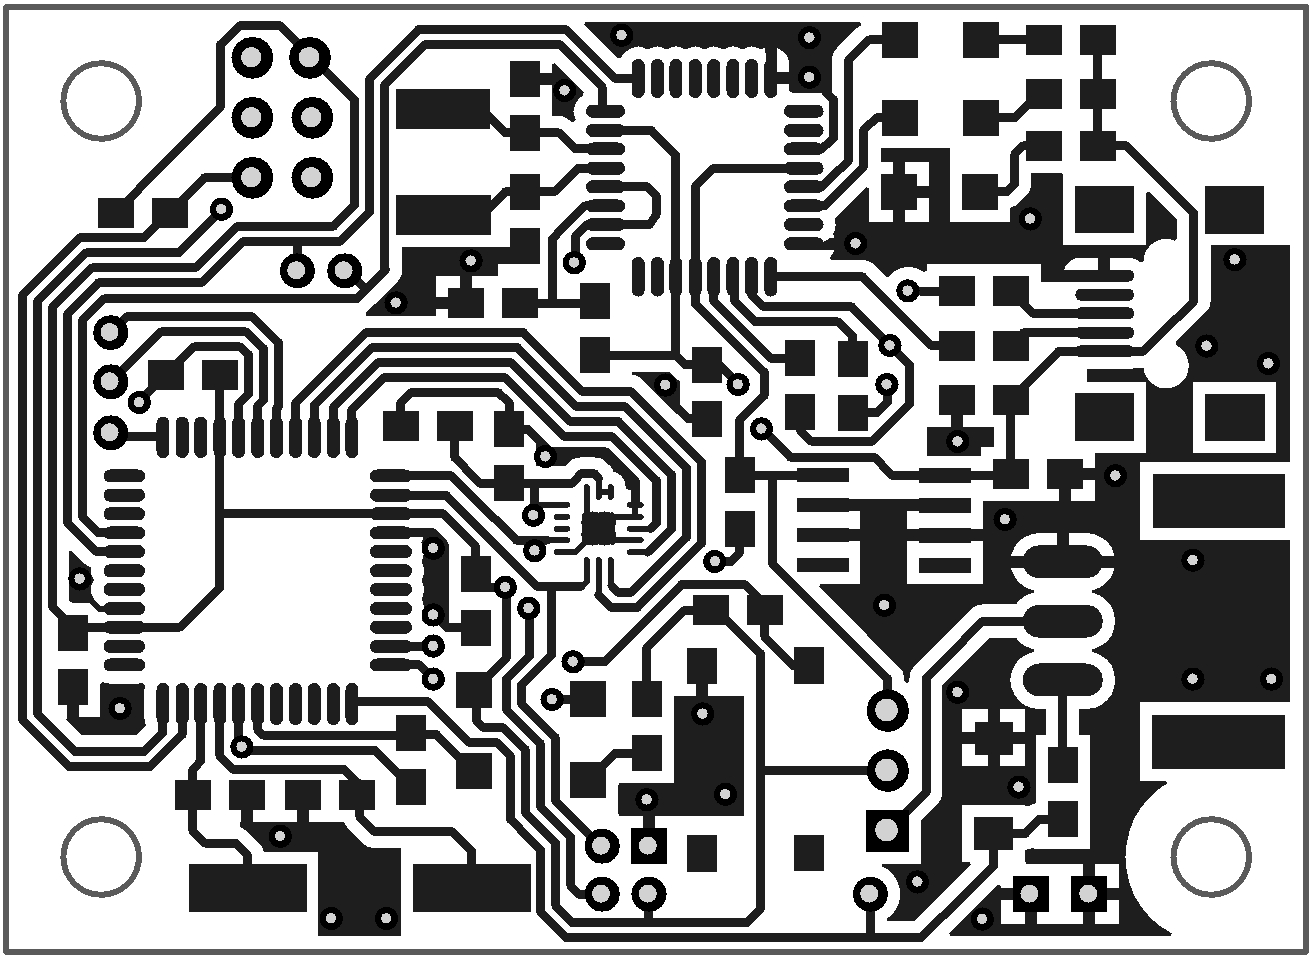
\includegraphics[width=7cm,]{img/HW/top.png}
		\caption{Top Layer}
		\label{fig:TopBot}
	\end{minipage}
	\hfill
	\begin{minipage}[hbt]{7cm}
		\centering
		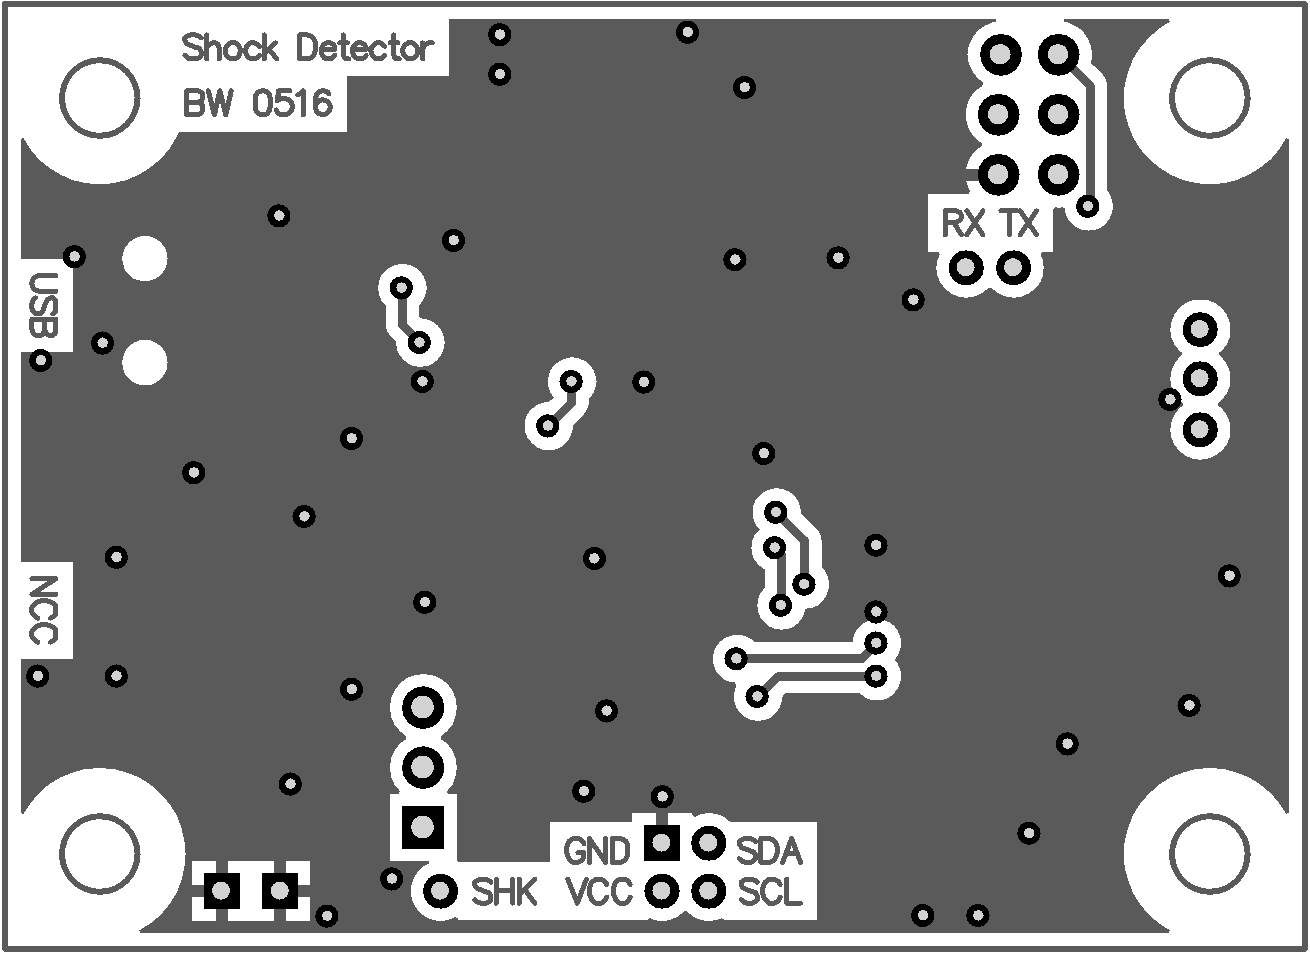
\includegraphics[width=7cm]{img/HW/bottom.png}
		\caption{Bottom Layer}
		\label{fig:TopBez}
	\end{minipage}
	\\[4ex]
	\begin{minipage}[hbt]{7cm}
		\centering
		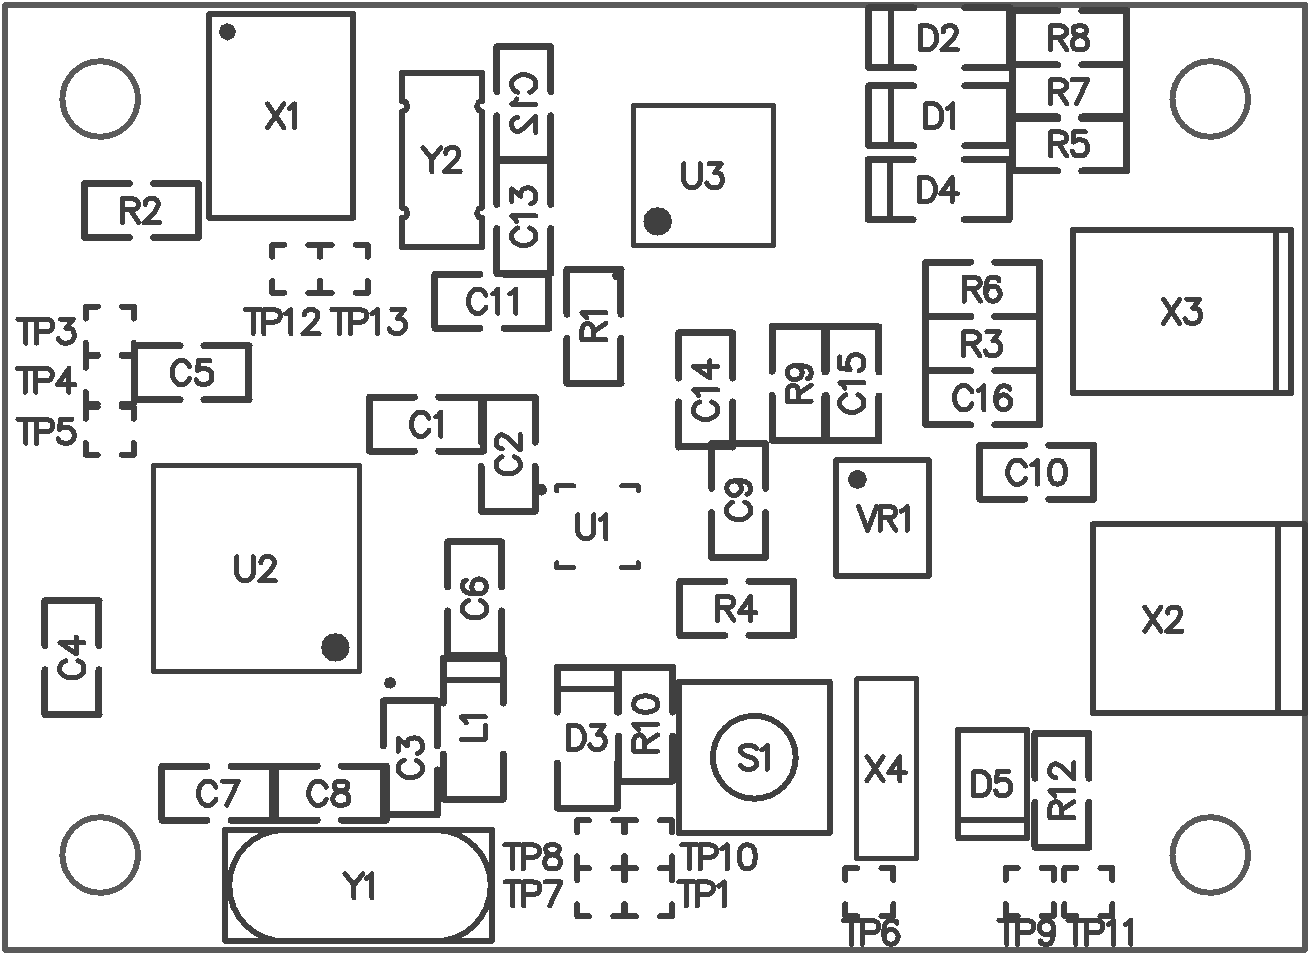
\includegraphics[width=7cm]{img/HW/designator.png}
		\caption{Bezeichnungen Top Layer}
		\label{fig:BotBez}
	\end{minipage}
	\hfill
	\begin{minipage}[hbt]{7cm}
		\centering
		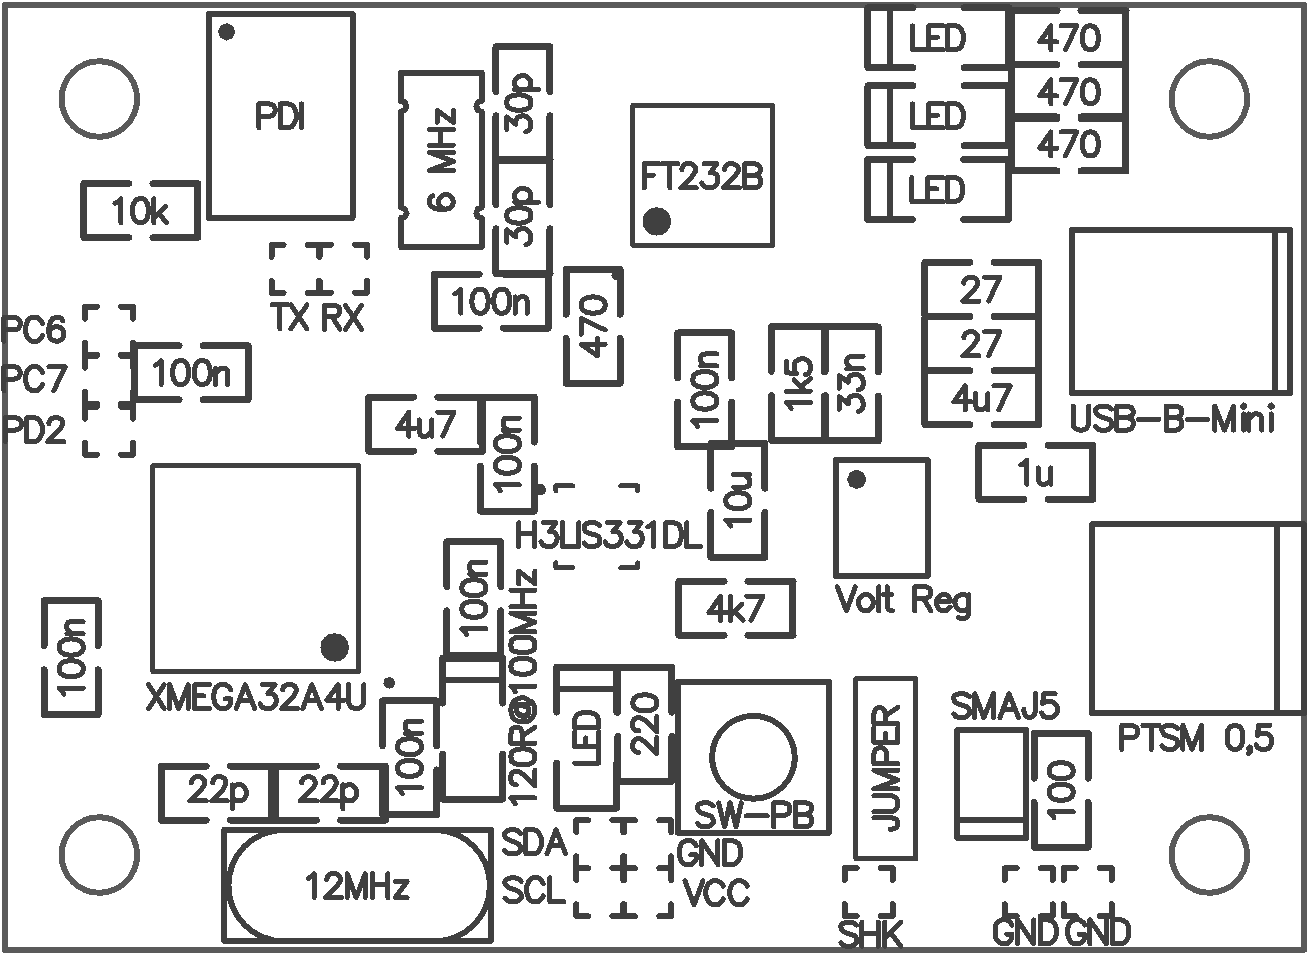
\includegraphics[width=7cm]{img/HW/comment.png}
		\caption{Werte Top Layer}
		\label{fig:BotVal}
	\end{minipage}
\end{figure}

\begin{figure}
	\centering
	%\vspace{-1cm}
	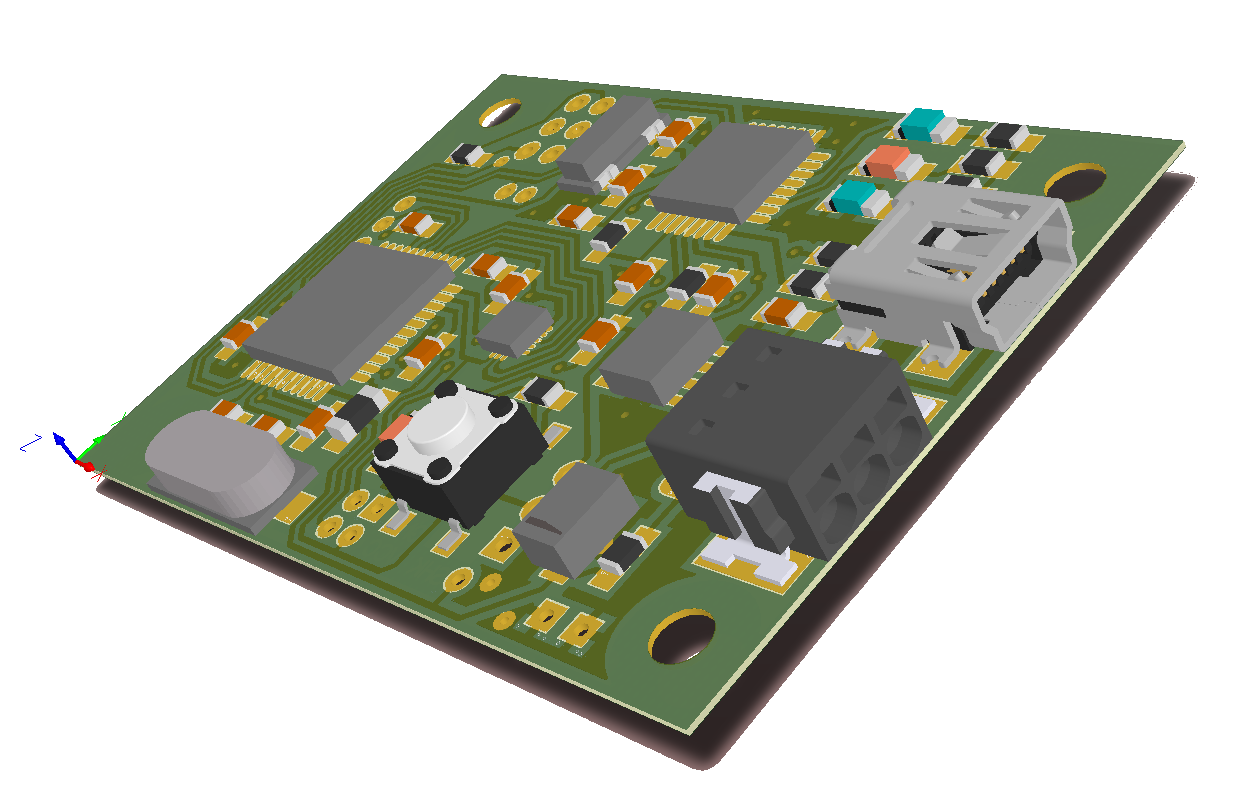
\includegraphics[width=13cm]{img/HW/3d_w.png}
	\caption{3D Ansicht des Printes}
	\label{fig:3d}
\end{figure}
